\documentclass[tikz,border=12pt]{standalone}
\usepackage{tikz}
\begin{document}
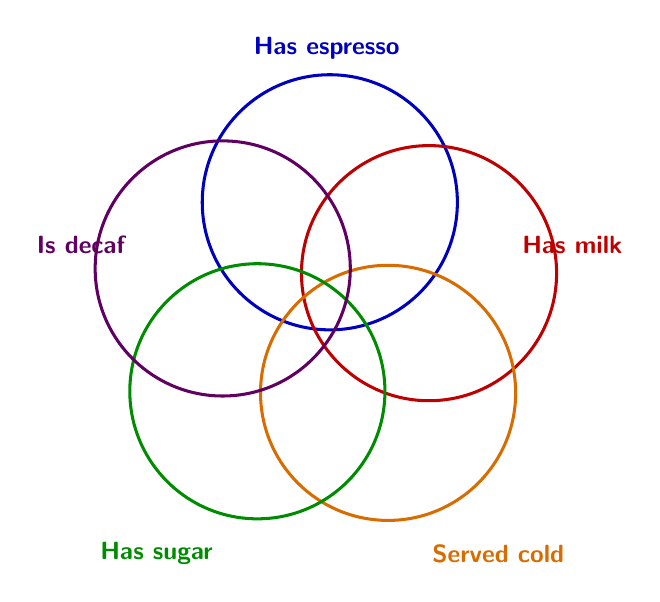
\begin{tikzpicture}[x=1cm,y=1cm]
  % General-position placement: every pair intersects.  Five circles can
  % form at most 22 planar regions (including the exterior), not 31.
  \def\radius{1.62}
  \draw[blue!75!black,line width=1.1pt] (0.04,1.32) circle (\radius);
  \draw[red!75!black,line width=1.1pt] (1.30,0.42) circle (\radius);
  \draw[orange!85!black,line width=1.1pt] (0.78,-1.10) circle (\radius);
  \draw[green!55!black,line width=1.1pt] (-0.88,-1.08) circle (\radius);
  \draw[violet!75!black,line width=1.1pt] (-1.32,0.48) circle (\radius);

  \node[font=\sffamily\bfseries\small,text=blue!75!black,align=center] at (0,3.28) {Has espresso};
  \node[font=\sffamily\bfseries\small,text=red!75!black,align=left] at (3.12,0.78) {Has milk};
  \node[font=\sffamily\bfseries\small,text=orange!85!black,align=center] at (2.18,-3.14) {Served cold};
  \node[font=\sffamily\bfseries\small,text=green!55!black,align=center] at (-2.16,-3.14) {Has sugar};
  \node[font=\sffamily\bfseries\small,text=violet!75!black,align=right] at (-3.12,0.78) {Is decaf};
\end{tikzpicture}
\end{document}
